\begin{figure}[H]
    \centering
    \begin{subfigure}{\textwidth}
        \centering
        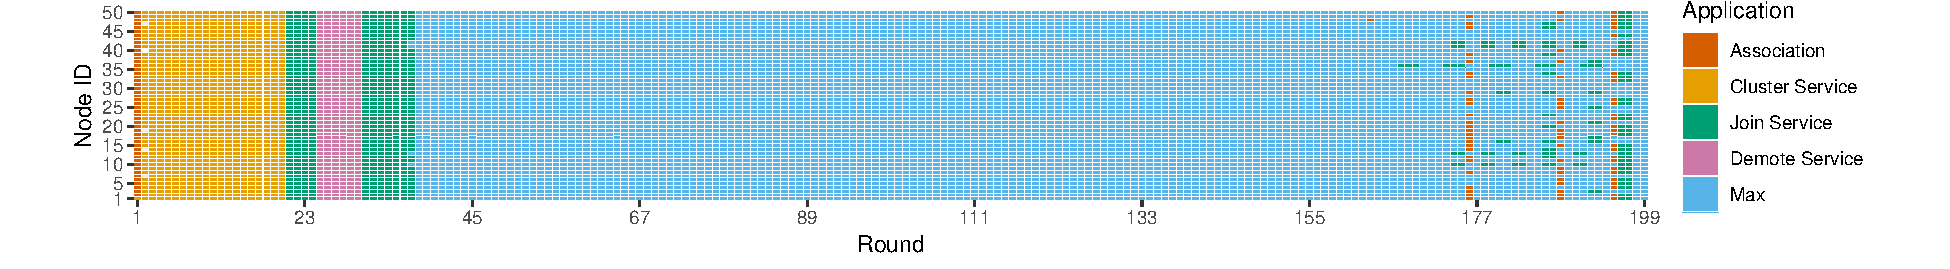
\includegraphics[width=\textwidth]{figure/Results/ReliabilityDiscussionApplicationHeatmaps/applicationmap50x50_1.pdf}
        \label{subfig:application-map-50-nodes-round-1-199}
    \end{subfigure}
    \hfill
    \begin{subfigure}{\textwidth}
        \centering
        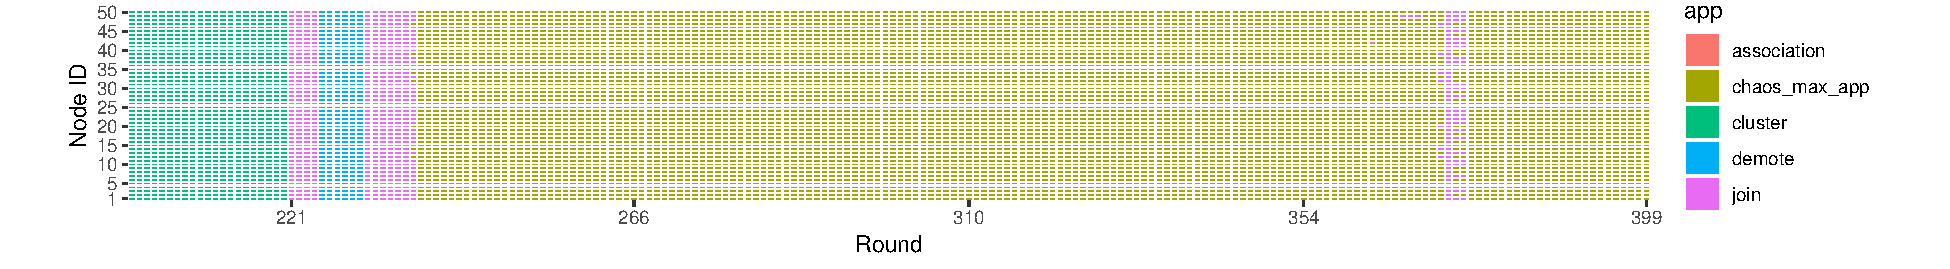
\includegraphics[width=\textwidth]{figure/Results/ReliabilityDiscussionApplicationHeatmaps/applicationmap50x50_2.pdf}
        \label{subfig:application-map-50-nodes-round-200-399}
    \end{subfigure}
    \begin{subfigure}{\textwidth}
        \centering
        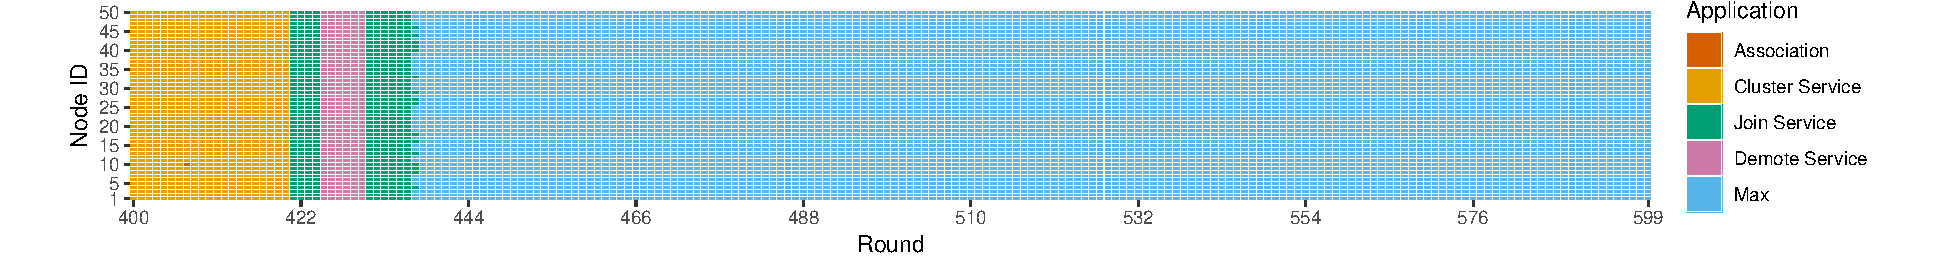
\includegraphics[width=\textwidth]{figure/Results/ReliabilityDiscussionApplicationHeatmaps/applicationmap50x50_3.pdf}
        \label{subfig:application-map-50-nodes-round-400-599}
    \end{subfigure}
    \caption{Application heat map of a test with 50 nodes over a 100x100 network area executing 600 rounds. Join is rarely executed outside its specified schedule.}
    \label{fig:application-map-50-nodes}
\end{figure}